\chapter{Introduction to Quantum Software}
\label{chpt:quantumsoftware}

%\epigraph{\textit{A new breed of quantum programmer is needed to study and implement quantum software — with a skillset between that of a quantum information theorist and a software engineer.}}{Will Zeng\\ Rigetti Computing \cite{WZ2017}}
%%%%%%%%%%%%%%%%%%%%%%%%%%%%%%%%%%

\addcontentsline{toc}{section}{2.0 \hspace{0.3cm}Introduction}

Now that we have introduced some quantum mechanics and how it can be connected to the idea of a computation using circuits and gates, we can start looking at how to write quantum programs. There are already various software packages available which are specifically designed to make interaction with a quantum computer easier, even though the quantum computers themselves are only just starting to get developed. Because of this, most software also includes simulators, which can either run on your computer at home or use more powerful computers via cloud computing. Next to that, some of the software can used with the quantum chips that have been developed by IBM, Google, Rigetti and D-Wave. However, the simulators are usually free, whereas access to these chips is often not. Furthermore, with the exception of D-Wave, which is a very specialised quantum computer, the chips are still very primitive and the simulators are just as suitable for you to develop a good understanding of quantum programming principles.

In this guide six different software packages will be used: pyQuil, QISKit, ProjectQ, Q\#, D-Wave Ocean and 1QBit. The first four are designed to be used for universal quantum computing, whereas the last two are more focused on optimisation problems.

In this chapter we will introduce these software packages, explaining their basic syntax and giving a minimal example quantum program: Create a qubit, put it in a superposition and then measure it, see example 1. Another example is used for D-Wave Ocean and 1QBit, as their general purpose is different. A brief overview of quantum software that is not more extensively considered in this guide is given is section \ref{FurtherLanguages}. At the end, we will include a short comparison between the software packages that have been introduced in this chapter.

In general quantum programs have three main steps:
\begin{enumerate}
    \item Allocate qubits
    \item Apply gates to single or multiple qubits
    \item Measure the final state of the qubits
\end{enumerate}
This structure is not 100\% accurate, as one may allocate additional qubits for certain steps of an algorithm, or measure part of the qubits before applying more gates to the leftover qubits before measuring them. However, one must always allocate some qubits to get started and the final step should always be a measurement, as the human-computer interaction will always be classical and we therefore need to get classical information from the qubits to be able to use to result of a quantum computation in any way.

Another thing one has to keep in mind is that quantum computers are very good at some specific tasks, but there are also many tasks where classical computers are just as good or even better. Classical computers have been around for a very long time and benefit from many optimisations that have been developed in this time. Therefore, when programming we should try and use classical and quantum computers together, each for the tasks they are best at, respectively. Some software packages do this explicitly, where different parts of your program apply to the classical CPU and the quantum processor (QPU). Other packages sort this out themselves and let the user just use qubits in the main program.

\subsection{Simple example}

%%%%%%%%%%%% title= Example 1
\begin{tcolorbox}[standard jigsaw,
    opacityback=0,  % this works only in combination with the key "standard jigsaw"
    boxrule=0.5pt,label={example0000001}]
    {\bf Example 1: Generating and measuring a single-qubit state}
    \tcbline
    Generate the one-qubit pure state 
    \begin{align*}
    \ket{\psi}=\frac{1}{\sqrt{2}}\left(\ket{0}+\ket{1}\right),
    \end{align*}
    by applying gates to the initial state $\ket{0}$ and then perform measurements.
\end{tcolorbox}
%%%%%%%%%%%%%%%


%%%%%%%%%%%%%%%%%%%%%%%%%%
\section{Rigetti - pyQuil}
%%%%%%%%%%%%%%%%%%%%%%%%%%

pyQuil is a Python based programming language created by Rigetti \cite{pyQuilDoc} as part of their quantum programming toolkit for their hardware. In this section we address the main features of pyQuil and the description of its syntax with a simple example. 

%%%%%%%%%%%%%%%%%%%%%%%%%%%%%%%%%%%%%%%%%
\subsection{Quantum Programs with pyQuil} 
\label{Quantum Programs with pyQuil}
%%%%%%%%%%%%%%%%%%%%%%%%%%%%%%%%%%%%%%%%%

%Quantum algorithms require the implementation of three computational stages. We first initialise the state to $\ket{00...0}$, then apply gates in order to obtain a target state of interest, and finally perform measurements in the computational basis. Let us see how to address these stages with the following specific example. 

We will now do a simple demonstration in pyQuil to create and measure the superposition $\frac{\ket{0}+\ket{1}}{\sqrt{2}}$. We will need to initialise a qubit in the $\ket{0}$ state, then apply a Hadamard gate and measure the result.\\

\noindent \begin{minipage}{0.45\textwidth}
%%%%%%%%%%%%%%%%%
\begin{minted}{python}
# 1. Calling Libraries
from pyquil.quil  import Program 
from pyquil.api   import QVMConnection 
from pyquil.gates import H
# 2. Initialising the program
qvm = QVMConnection()
p = Program()
# 3. Applying gates
p.inst(H(0))
# 4. Performing measurements
p.measure(0,0)
# 5. Executing the program
results = qvm.run(p, [], 4)
print(results)
\end{minted}
%%%%%%%%%%%%%%%%
\end{minipage} \hfill
%
\begin{minipage}{0.55\textwidth}
%    \hspace{0.5cm} Walking through example \autoref{lst:ExampleQVM} step by step:
\begin{enumerate}
    \item \textbf{Calling libraries} - We call an object Progam which will contain the instructions of our program, a connection to the QVM and the single-qubit gate Hadamard $H$. 
    \item \textbf{Initialising the program} - When allocating a program (p in this case) we implicitly have allocated $n$  qubits in the state $|00...0>$. The amount of available qubits will depend on whether it's being run on a QVM or a QPU. The object program will contain the list of instructions to be run later on.
\end{enumerate}
\end{minipage}
%%%%%%%%%%%%%%
\begin{enumerate}
\setcounter{enumi}{2}
\item \textbf{Applying gates} - Considering the method isnt we apply from left to right in order of application and inside parenthesis the qubit which is acting upon the qubits are listed from $0,1,...n$. For instance applying Hadamards for two qubits the notation is this. The complete set of gates can be found in HERE. and u can define your own gates in the following way:
    \item \textbf{Performing measurements} - We add the instruction measuring qubit zero and assigning it to classical register 0 and similarly for qubit 1.
    \item \textbf{Executing the program} - The object program p is a list of instructions which are now being run. We print the results.
\end{enumerate}

%Example code for running the same code on the real QPU.

\begin{comment}
%We would like to implement this in a real quantum computer, and this is where Rigetti comes in. We need further software to manipulate real QPUs, and therefore cannot be as straightforward as our previous code. but we are using the QVM.

%\columnbreak

{\bf 0. Libraries:} The connection and qubit initialisation of our qubits is given by:
\begin{lstlisting}[language=Python]
from pyquil.quil  import Program 
from pyquil.api   import QVMConnection 
from pyquil.gates import I,X,Z,Y,H,PHASE
import numpy as np
\end{lstlisting}

{\bf 1. Initialisation:} The systems has been initialised into a state of $n$
 qubits in the $|00...0>$ state. Of course both the qvm and qpu are limited by this and that respectively.\\ 
 
 the other point is that this is a lst of instructions and the actual computation has not taken place, and we need to invoke the command run to do it.\\
\begin{lstlisting}[language=Python,firstnumber=5] 
# Invoking and renaming
qvm=QVMConnection()
p=Program()
\end{lstlisting} % numbers=none 
 
 %%%%%%%%%%%%%%%%%%%%%%%%%%%%%
 {\bf 2. Gate implementation:} So far we have only covered initialisation, now we need to consider state manipulation. The way that gates are being called is as follows:
 %%%%%%%%%%%%%%%%%
\begin{lstlisting}[language=Python,firstnumber=8]
# Gate implementation
p.inst(H(0))
theta=np.pi/2
\end{lstlisting}
%%%%%%%%%%%%%%%%
 by considering the object program which we have renamed as p with the methd isnt we apply fro left to right in order of application and inside parenthesis the qubit which is acting upon the qubits are listed from $0,1,...n$. For instance applying gates this and that. The complete set of gates can be found in HERE.\\
 
%%%%%%%%%%%%%%%%%%%%%
{\bf 3. Measurement:} Yadda describing 
\begin{lstlisting}[language=Python]
# Measurement
p.measure(0,0)
p.measure(1,1)
\end{lstlisting}

Here interlude printing P and linking this to the compiler.
 
%%%%%%%%%%%%
{\bf 4. Run:} So far this is only a list, now finally we run the program with the command.
\begin{lstlisting}[language=Python]
# Running the program
cr=[]
results=qvm.run(p,cr,4)
print(results)
\end{lstlisting}
\end{comment}
%%%%%%%%%%%%

%%%%%%%%%%%%%%%%%%%%%%%%%%%%
\section{IBM - QISKit}
%%%%%%%%%%%%%%%%%%%%%%%%%%%%

\begin{comment}
IBM has launched the IBM Q experience that consists of a development environment called QISKit, a higher-level gate-building software development kit (SDK) that allows users to compose their own quantum algorithms, and OpenQASM, a low level quantum assembly language to realise the gates at the quantum prosessing unit (QPU). 

There is ample space for development of algorithms in this environment as the visual arrays provide a clear structure to those familiar with quantum computation. The composer also displays the code on which it operates so that users interested in further development have the opportunity to learn how to code their own gates in OpenQASM as well as QISKit. The associated documentation which is linked on the IBM Q website provides more detail to the structure \cite{coles2018quantum}. 

The architectures (physical or virtual) that the user can execute their quantum algorithms on are easily accessible via the IBM Q Experience web page. IBM recently published a report detailing their state-of-the-art prototype 50 qubit chip in the 2017 IEEE ICRC conference \cite{ibm50}.
\end{comment}

%%%%%%%%%%%%%%%%%%%%%%%%%%%%%%%%%%%%%%%%%
\subsection{Quantum Programs with QISKit}

Our first example using QISKit is to generate a single qubit superposition, $\ket{\psi}=\frac{1}{\sqrt{2}} \left(\ket{0}+\ket{1}\right)$.

We can simulate both of these actions on the composer in the IBM Q experience, or use experiment tokens to run the program on the processor IBM provides (referred to as ibmqx4) as seen in \autoref{fig:H}. 

\begin{figure}[h!]
    \centering
    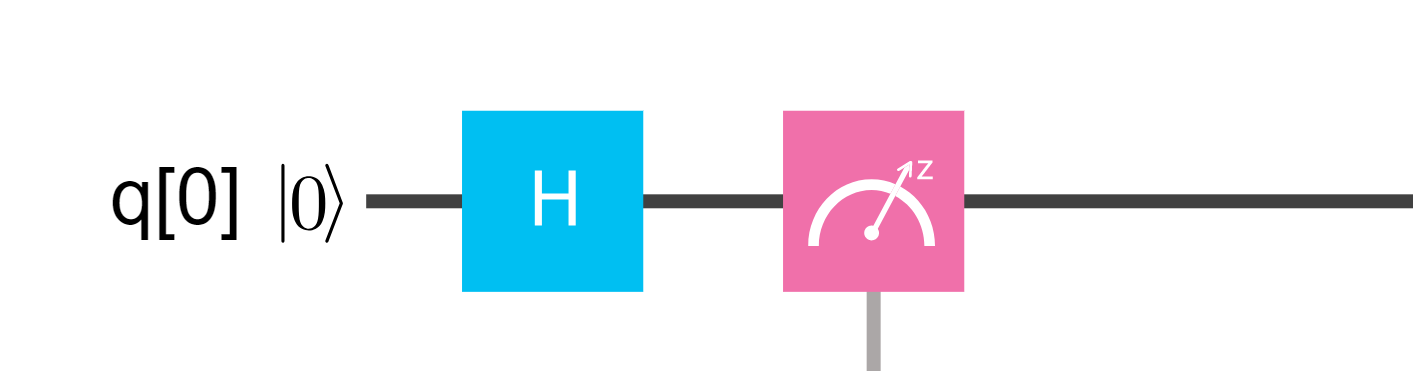
\includegraphics[width=00.5\textwidth]{Hcodecomposer}
    \caption{The composer view of the code that we can use to simulate the generation of $H\ket{0}=\frac{1}{\sqrt{2}}\left(\ket{0}+\ket{1}\right)$.}
    \label{fig:H}
\end{figure}

Though the composer is a useful place to get started with your own simulations of basic gate operations, it doesn't give us a an opportunity to truly experiment with the hardware at a deeper level. To do this, we need to start experimenting with the QISKit language itself.

To create this state, and measure it on IBM's Q QASM Simulator,

\inputminted{python}{code/QISKit/superpos_qiskit.txt}

When run, the output produced is as follows:

\begin{minted}{python} 
Local backends:  ['local_qasm_simulator', 'local_statevector_simulator', 'local_unitary_simulator']
simulation:  COMPLETED
{'0': 528, '1': 496}
\end{minted}

Here, the back end in selected in line 1, completion confirmation is shown in line 2, and the measurement basis and counts are shown in line 3, illustrating that indeed the Bell State specified in \autoref{eq:BS} has been generated, and measured. 

%%%%%%%%%%%%%%%%%%%
\section{ProjectQ}

ProjectQ is an open source domain specific language embedded in Python. ProjectQ can run on a local simulator - your computer. But there is also an option to connect to the IBM back-end to run code on their simulator or chips, and this may be extended to other hardware in the future as well. This makes ProjectQ a general quantum programming language that is not platform specific unlike pyQuil and QISKit.  



% Note: This section is not finished! I will complete the compiler paragraph and discuss the different back-ends etc. 

%%%%%%%%%%%%%%%%%%%%%%%%%%%%%%%%%%%%%%%%%%%
\subsection{Quantum Programs with ProjectQ}
%%%%%%%%%%%%%%%%%%%%%%%%%%%%%%%%%%%%%%%%%%%

% I may add another example to this section since it is quite short. Or do things need explaining in more detail?

We will now do a simple demonstration in ProjectQ to create and measure the superposition $\frac{\ket{0}+\ket{1}}{\sqrt{2}}$. We will need to initialise a qubit in the $\ket{0}$ state, then apply a Hadamard gate and measure the result.

\inputminted{python}{code/ProjectQ/superpos_projectq.txt}

Walking through this example step by step,

\begin{itemize}
    \item \textbf{Initialising the program} - The first thing to do is to set up the back-end that the program will be run on. This is done by calling \texttt{MainEngine} which has the local simulator (your computer) as default, this can also be set up to be the IBM back-end or something else such as a circuit drawer.
    \item \textbf{Allocating qubits} - Qubits can now be allocated, either individually (as shown above) or as a register, from the \texttt{engine}. Creating a single qubit is done using \texttt{allocate\_qubit} and a register by \texttt{allocate\_qubit(n)}.
    \item \textbf{Applying gates} - The syntax to do an operation is  \texttt{Gate | Qubits}. 
    \item \textbf{Performing measurements} - Measurements have the same syntax as applying gates but using the command \texttt{Measure}. It is really important to measure all your qubits at the end of the program to avoid errors in your code.
    \item \textbf{Executing the program} - The gates are sent to the back-end by use of the \texttt{flush} command. If you wish to display the result, the qubit can be converted to type integer after measurement.
\end{itemize}

%%%%%%%%%%%%%%%%%%%%%%%%%
\section{Microsoft - Q\#}
%%%%%%%%%%%%%%%%%%%%%%%%%

One of the languages that is strongly quantum platform independent is Q\#. It is being developed by Microsoft and very roughly based on their classical languages C\# and F\#. It is, however, not just a library, but designed to be its own language. Q\# is developed to be a high-level quantum programming language. Though it still allows the basic single qubit operations, it also provides a more advanced library and allows user-defined ``operations" which can be used to structure more complicated programs. The programming language should be platform independent to allow users to write programs now for quantum computers available in the future. Currently it runs on a simulator (either on your local computer or Azure, a Microsoft cloud computing service) or a cost estimator (trace simulator) which approximates qubit and gate requirements for the program. 

The concept behind the language is that the quantum computer is treated like a coprocessor: like a GPU is a graphical coprocessor, a QPU is the quantum one. This means that a program using the QPU requires a driver program, which controls the main processor (CPU) and which then calls on a subprogram controlling the QPU. The QPU program in this case will be written in Q\#, whereas the driver program can be written in not just C\# or F\#, but any language supporting the .NET framework. In this programming guide the driver programs are written in C\#, but you could easily change this if you are more comfortable with another language.

As Q\# is dependent on the .NET framework, it is currently only available for computers having this framework installed. This is no longer restricted to Windows computers, but a version of the .NET framework has recently become available for Mac and Linux computers as well. The easiest way to get started is probably by programming with Visual Studio, as it has inbuilt .NET support. Tutorials for installing this API and Q\# can be found online. 

Q\# comes with a standard library which is divided into two sections: The basic building blocks of the language, such as the qubit and measurements representations and the operations given above, are part of the so-called prelude. The prelude is dependent on the target machine, e.g. a simulator.  The second part, called the canon, is machine independent and built on the elements that form the prelude. It gives implementations of various quantum algorithms such as a quantum Fourier transform and a phase estimation.  

\paragraph{Basic building blocks} There are several primitive types specific to Q\# and an overview of these is given in table \ref{table:PrimTypeQsharp}. The first five are analogous to types in classical programming languages, e.g. C\#. The others are more quantum programming specific. 

It is also possible to create arrays, e.g. a \texttt{Qubit[]} or an \texttt{Int[][]}. Tuples, so e.g. (a, b, c), are also used. a, b and c could be of different types and tuples can be quite useful in returning multiple values from an operation. You can also define your own types, but they must be based on the primitive types.

Another thing a Q\# programmer has to keep in mind, is that variables are normally immutable. Values are assigned with a \texttt{let} statement and they cannot be changed afterwards. To allow changing the value of a variable one can use the \texttt{mutable} keyword when assigning a value to a variable. Changing the variable is then done with the \texttt{set} statement.

Qubits are maybe the most important resource in a quantum program. You cannot assign a value to a \texttt{Qubit}, but you can measure it and then apply operations to change it to the value you want. The default value of a \texttt{Qubit} is $\ket{0}$, i.e. the computational \texttt{Zero} state, and it is generally good practice to reset a used \texttt{Qubit} to this before releasing it.

The easiest way to use actually use \texttt{Qubit}s is to write a \texttt{using} statement, e.g. \texttt{using (qubits = Qubit[2])\{<any code using these qubits>\}}.

\begin{table}[!htb]
      \centering
        \begin{tabular}{|l|l|}
        \hline
        Type    & Values \\ 
        \hline
        \texttt{Int}     & 64-bit signed integer \\
        \texttt{Double}  & double-precision floating-point number \\
        \texttt{Bool}    & Boolean value (\texttt{true} or \texttt{false}) \\
        \texttt{String}  & Unicode sequence, used to pass messages to classical driver program\\
        \texttt{Range}   & sequence of integers\\
        \texttt{Qubit}   & qubit\\
        \texttt{Result}  & outcome of measurement (\texttt{One} or \texttt{Zero})\\
        \texttt{Pauli}   & elements of the Pauli group (\texttt{PauliI}, \texttt{PauliX}, \texttt{PauliY} or \texttt{PauliZ})\\
        \hline
    \end{tabular}
    \caption{Primitive types in Q\#}
    \label{table:PrimTypeQsharp}
\end{table}

%%%%%%%%%%%%%%%%%%%%%%%%%%%%%%%%%%%%%%%%%
\subsection{Quantum Programs with Q\#}
%%%%%%%%%%%%%%%%%%%%%%%%%%%%%%%%%%%%%%%%%
Q\# programs require two main bits of code: a ``classical" driver program and the quantum program. The driver program here is in C\#, but as mentioned in the previous section this could be another language. It must use two namespaces: \texttt{Microsoft.Quantum.Simulation.Core} and \\ \texttt{Microsoft.Quantum.Simulation.Simulators}. Next you want to define the namespace you want to work in: in this case Quantum.Superposition, which will be shared by your driver and your quantum program. A namespace is way to define a scope that can contain different elements in a program. The namespace can span multiple files and, as in our case, can be used by different languages.

Then you start your driver program like you would any regular program. In C\# you create a class and the entry point for the program is your \texttt{static void Main(string[] args)} method.

As we do not have an actual QPU, we are using a simulator. To create an instance of the simulator in your program you can use a \texttt{using} block. This creates the simulator instance and ensures it is disposed of when the block ends.

In the "using" block you can then call on the quantum operation defined in your quantum subprograms. In this case that will be the operation "Superposition". The operation is actually run with the method \texttt{Run(<QuantumSimulator>, arg1, arg2, ...)}, where the \texttt{arg} arguments are any potential arguments passed to the quantum operation. In this simple example the quantum operation does not take any arguments so we are only passing the Quantumsimulator \texttt{sim} to \texttt{Run}. Finally, we want to actually get the outcome of the quantum operation, which we get by adding \texttt{.Result} to the end.

Then the rest of the driver program can be completely classical again, with the exception that the objects returned can be specific quantum types.

\begin{listing}[H]
\begin{minted}{csharp}
using Microsoft.Quantum.Simulation.Core;
using Microsoft.Quantum.Simulation.Simulators;

namespace Quantum.Superposition{

    class Driver{
        static void Main(string[] args){

            using (var sim = new QuantumSimulator()) {
                Result outcome = Superposition.Run(sim).Result;
                System.Console.WriteLine
                        ($"Measuring equal superposition state gave outcome {outcome}.");
            }

            System.Console.WriteLine("Press any key to continue...");
            System.Console.ReadKey();
        }
    }
}
\end{minted}
\caption{Starting a driver program for Q}
\label{lst:CdriverSimple}
\end{listing}

To specify the quantum operation you need to write Q\# code. Again, you start by defining the namespace we are working in (\texttt{Quantum.Superposition}). Next there are two namespaces you will need to use, which are specified with the keyword \texttt{open} (similar to \texttt{using} in C\#): \\ \texttt{Microsoft.Quantum.Primitive} and \texttt{Microsoft.Quantum.Canon}.

New operations are defined with the keyword \texttt{operation} and the arguments taken and the return value is specified here in the form \texttt{operation OperationName (arg1: type1, arg2: type2, ...) : (returnType)}.
Inside the operation you define the actual steps to take in the \texttt{body} block. 

Here we are defining a mutable variable res. It is assigned the value \texttt{Zero}, which is of type \texttt{Result}. This variable will be used to return the outcome of the quantum operation. Next, a \texttt{Qubit} array containing one \texttt{Qubit} is created and after applying a Hadamard (\texttt{H}) gate the \texttt{Qubit} will be in state $\frac{\ket{0}+\ket{1}}{2}$. Then the \texttt{Qubit} is measured (\texttt{M}) and afterwards returned to the $\ket{0}$ state. The measurement outcome is then returned to the driver program. 

One thing to note here is that we needed to define the variable \texttt{res} outside the \texttt{using} block, as any variables defined in the block are local only to the \texttt{using} block. We cannot use the return statement inside the \texttt{using} block either, so we needed to use a variable local to the whole \texttt{body} block to return a value from the operation.\\

\begin{listing}[H]
\begin{minted}{fsharp}
namespace Quantum.Superposition{

    open Microsoft.Quantum.Primitive;
    open Microsoft.Quantum.Canon;

    operation Superposition() : (Result){

      body{

        mutable res = Zero;

	    // create a qubit reqister
	    using (reg = Qubit[1]){
	      // Apply the Hadamard gate to your qubit to create an equal superposition
            H(reg[0]);

	      // Measure the qubit in superposition
	      set res = M(reg[0]);

	      // Reset the qubit to its clean |0> state
	      if (res == One){
	        X(reg[0]);
	      }
	    }

      return res;
            
      }
    }
}
\end{minted}
\caption{A simple program in Q creating and measuring an equal superposition.}
\label{lst:QSimple}
\end{listing}


%%%%%%%%%%%%%%%%%%%%%
\section{D-Wave-Ocean}
%%%%%%%%%%%%%%%%%%%%%
%%%%%%%%%%%%%%
\begin{comment}
\begin{itemize}
    \item Syntax
    \item Simple example
    \item explaining that the types of problems being addressed by Dwave are different than the ones from the other libraries/languages
\end{itemize}
\end{comment}
%%%%%%%%%%%%%

As the universal quantum computer is hard to achieve in the short term requiring high quality and scalable qubits, the technologies presented here make use of existing qubits as an intermediate step towards the goal of universal quantum computing. One of these technologies is quantum annealing.

 Different from universal quantum computer which can implement algorithms by gate, annealing type quantum computer is ansatz based computer designed for specific optimisation problem. Annealing is a process that searches for the minimum energy of a state. Classically this is done by the thermal annealing (simulated annealing) changing the configuration slowly and accepting the configuration when lower energy state is achieved. Quantum annealing is expected to be implemented more efficiently with the assistance of entanglement and tunneling as showed in \autoref{fig:Tunnelling}.\\
 
 \begin{figure}[h!]
    \centering
    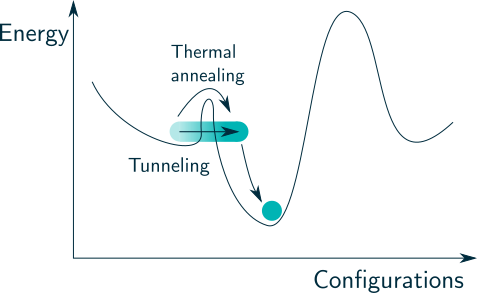
\includegraphics{figures/Tunneling.png}
    \caption{Caption}
    \label{fig:Tunnelling}
\end{figure}
 

  D-wave has its own software stack:
  
\begin{itemize}
    \item \textbf{D-Wave Ocean}- D-Wave toolkits to help solve problems on D-Wave system.
     \item \textbf{qbsolv}- Open source hybrid optimization solver for partitioning quadratic unconstrained binary optimization (QUBO) problems which is ran either on tabu classical solver or D-Wave system. By default, the classical solver is used. To use D-Wave's machine, separate arrangements should be included.
    \item \textbf{QPU}- Quantum processing unit. An API key is needed to run the program on the quantum computer.
 \end{itemize}
Here as an example we will consider getting the configuration to minimise the quadratic polynomial $-x_0-x_1+2x_0x_1$ for \ $x_i\in\{0,1\}$  

\begin{minted}{python}
import dwave_qbsolv

# Create a quadratic polynomial -x_0 - x_1 + 2x_0x_1 
Q = {(0, 0): -1, (1, 1): -1, (0, 1): 2}

# Create the local solver
solver = dwave_qbsolv.QBSolv()

# Solve for the minimum energy configuration
response = solver.sample_qubo(Q, num_reads=300) # Sample 300 times
sol = list(response.samples())
energy = response.data_vectors['energy']
print(sol)
print(energy)
\end{minted}
The output gives
\begin{minted}{python}
[{0: 1, 1: 0}, {0: 0, 1: 1}]
[-1. -1.]
\end{minted}
It can be seen that $x_0$ and $x_1$ will always take different value. This is equivalent to the NOT logic. 
Generally, the Boolean gate can be implemented as the QUBO form. 

%%%%%%%%%%%%%%%%%%%%%%%%%%%%%%%%%
\section{1QBIT-QUANTUM-READY SDK}
%%%%%%%%%%%%%%%%%%%%%%%%%%%%%%%%%

Alternatively, 1Qbit has developed the 1QBIT QUANTUM-READY™ software development kit targeting hardware independent languages. Currently it uses a local classical solver or interface with D-Wave's system via an API key. Both the 1QBIT SDK and D-Wave Ocean stack can be run with Python.
We will introduce the 1QBIT QUANTUM-READY™ SDK in this section, as an example of the language used to interface with D-Wave's machine. Currently, only online Jupyter Notebook versions of the language are available \textit{(see \url{http://qdk.1qbit.com/})}.
By default a classical solver is used. To use D-Wave's machine, separate arrangement should be made.\\
\begin{minted}{python}
from qdk import *

# Create a quadratic polynmial  -x_0 - x_1 + 2x_0x_1  
builder = QuadraticBinaryPolynomialBuilder() 
builder.add_term(-1.0, 0, 0) 
builder.add_term(-1.0, 1, 1) 
builder.add_term(2.0, 1, 0)  
qubo = builder.build_polynomial()

# Create a local solver 
solver = DWaveSolver()

# Get configuration of best solution 
solver.solver.num_reads = 300 # Sample 300 times
sol = solver.minimize(qubo)
print(sol) 
\end{minted}
The output is
\begin{minted}{python}
Energy = -1, Frequency: 152, Configuration = {x0 = 0, x1 = 1}
Energy = -1, Frequency: 148, Configuration = {x0 = 1, x1 = 0}
\end{minted}
%%%%%%%%%%%%%%%%

%%%%%%%%%%%%%%%%%%%%%%%%%%%%%%
\section{Comparison of Languages}

We now compare some of the implementation dependent features of the languages and give a comparison between them.

pyquil
qubits are denoted by integers which can be unclear sometimes.

qiskit 
%%%%%%%%%%%%%%%%%%%%%%%%%%%%%%%%%%%%%%%%%%%%%%%%%%%%%%%%5
\subsubsection{General syntax comments}


PyQuil has nice syntax handling of gates \texttt{program.inst(gate\_1(qubit\_1, gate\_2(qubit\_2)}

Qiskit syntax is ok. the documentation is rather difficult to find in some of the examples we mention here \footnote{Can we say this?}\footnote{The documentation is impossible, there are random links everywhere to depreciated methods...}

Project Q has a heavy focus on making the programs written using it to look (syntactically) like operators acting on states. The emphasis on Dirac notation is clear as the operation perform an Pauli X on qubit 1 is given by \texttt{ X | q[1]}.

%%%%%%%%%%%%%%%%%%%%%%%%%%%%%%%%%%%%%%%%%%%%%%%%%%%%%%%%5
\subsubsection{Qubit management}

The pyQuil qubit management is dynamic, qubits are allocated dynamically which does not require the users input but do have to allocate classical registers. 

The qiskit library is heavily based on using quantum circuits. You specify quantum and classical registers and ancilla qubits. 

Project Q also requires the user to manually allocate qubits and the QASM resembles dynamically allocated qubits with allocate and deallocate at the start and end of the instruction set. 

Q\# using to allocate qubits but don't have to declare classical variable but c\# is typed.
%%%%%%%%%%%%%%%%%%%%%%%%%%%%%%%%%%%%%%%%%%%%%%%%%%%%%%%%5
\subsubsection{Compilers/Gate simplification}

All of the libraries have access to the standard gate set in their python environments\footnote{X,Y,Z,H,Phase gates and arbitrary rotations}. 

In pyQuil the user can also use the \texttt{defgate()} method to define their own gate either in terms of compositions of existing gates or by specifying a matrix representation of the gate. Qiskit also can define gates. Project Q has the option to define gates?


The pyQuil compiler takes one of Rigetti's quantum devices as an argument and compiles their Quill QASM into device specific gate-set and remaps the qubits to match the connectivity of the machine.

IBM has no working compiler\footnote{there is a compiler but it does nothing, specify x only and the program crashes, specify x and H and the program uses Z. U(x,y,z)($\theta$).} but we can return the Open QASM (IBM's Quantum Assembly format), 

The Project Q compiler is designed to have a modular structure, so the user can pick and choose the level of optimisation required. It works quite well although you have to manually specify the available gate-set you have access to and the connectivity of the machine. They are working on adding in backend support for the IBM quantum devices.


%%%%%%%%%%%%%%%%%%%%%%%%%%%%%%%%%%%%%%%%%%%%%%%%%%%%%%%%5
\subsubsection{Backends}

Rigetti then offers a remote Quantum Virtual Machine (QVM) which runs simulations of up to 26 qubits requiring an API key to use. They do not provide a local simulator which runs on a personal computer. IBM do provide a local simulator and access to their devices and remote simulator require and API key. Project Q comes with a local simulator, written in c++ and is built on your machine on install using python wrappers.

The project Q simulator is best of the local simulators however currently there is no way to compile project Q code into IBM's OASM to run on IBM's machines or compile to Quil to run on Rigetti's machines. Although IBM and Project Q existed as part of the same project \footnote{see git change-log} we are unsure of when the project Q to IBM backend will be implemented. 

One slightly annoying feature of pyQuil the software package is the lack of local quantum simulator. This can cause problems when trying to execute large programs as we often found the connection timed out before the program finished. 

%%%%%%%%%%%%%%%%%%%%%%%%%%%%%%%%%%%%%%%%%%%%%%%%%%%%%%%%5
\subsubsection{Device mappings}

Rigetti's Quil compiler takes a dictionary of one of their devices which then creates a map of the positions of the qubits and the connectivity of the machine. 

QISKits' \texttt{get remote backends} method doesn't return any valid devices to compile to, when using one of their device names an error saying the device is not valid is produced. It may be possible to manually add device mappings but even then the \textit{compiler} didn't compile to the given gate-set or it would produce an error for some gate-sets.

Project Q lets you specify the connectivity using a Python dictionary and gate-set by importing the gates you want/have access to. The compiler works quite well.

I think we should talk about the pros and cons of each language, to give the readers an idea of which one better fits their needs? \autoref{tab:mother}
\begin{itemize}
    \item {\bf Language-based?} Three of them are python-based, Q\# is not python-based
    \item {\bf Open source?} all of them are open source (which is good, I think)
    \item {\bf QPU?} pyquil, qiskit, project Q have access to QPU, Q\#? (could anyone confirm this?) although u need to request access to this.
    \item {\bf how beginner-friendly is the syntax?}
    \item {\bf particular conveniences} easy to implement oracles? qft?!!!!! what other conveniences?
    \item what other general characteristics should we highlight?
\end{itemize}

%%%%%%%%%%%%%%%%%%%%%%%%%%%%%%%%%
\section{Further languages} 
\label{FurtherLanguages}
%%%%%%%%%%%%%%%%%%%%%%%%%%%

There are a few languages and python libraries that haven't been mentioned in this guide due to differences in the computation model they are based on and their usefulness for immediate quantum programming. Some companies that aim to deliver full stacks of quantum software resources have not released any documentation, yet. Examples of these kinds of languages, libraries and resources are included below. 
\begin{itemize}
    \item \textbf{Scaffold} is a language that resembles the C and C++ programming languages and aims to provide structure in order to use classical variables and quantum registers in the same code, hence its name. Potential issues with memory allocation are reduced within the language, while allowing users to compose their relevant variables together. Several design decisions are included in the documentation to make programming easier. These include an imperative programming model (rather than a functional one) and rigorous error checks. Further reading can be found in the Scaffold publication \cite{Javadi2012}. 
    \item \textbf{Cirq} is an open-source project from Google that has recently been developed. The aim is to make quantum algorithms for existing quantum computers easier to code. Based on a python library, it allows simple tasks to be run on a simulated quantum processor, that will be available soon. Future access to Google's recently announced Bristlecone processor \cite{NISQ} will form part of this development package \cite{Cirqbristlecone}. Existing documentation and tutorials can be found at \cite{Cirq}.
    \item \textbf{Quipper} is a functional programming language for quantum computation that uses a high-level structure for gate organisation and programmable transformations of quantum circuits. As well as including all well-known quantum algorithms (like the ones we have mentioned), its distribution also includes seven operations from literature that are uncommon in other quantum software distributions. A full list of documentation and updates can be found on the Quipper website \cite{Quipper}.   
    \item \textbf{Strawberry Fields}, a full-stack continuous variable quantum software platform using Python. It relies on a completely different model of quantum computing where continuous variables replace discrete variables. The strawberry fields Python library allows access to the various elements of the stack. The quantum programming language named Blackbird is used to write quantum circuits inside of strawberry fields library. Blackbird uses similar syntax to Project Q but adapted to a continuous variable implementation. An example using both of these found in the quantum teleportation tutorial on the Xanadu website (see \cite{Strawberryfieldsteleportation}). The strawberry fields stack also includes an interactive  model for its quantum algorithm construction. More detail on these aspects can be found in the Xanadu whitepaper \cite{Xanadu2018}.
\end{itemize}
As mentioned before, a GitHub page has been dedicated to this topic that includes links to the relevant pages associated with quantum software: \cite{QuantumSoftwareList}. 
%%%%%%%%%%%%%%%%%%%%%%%%%%%

\newpage
%%%%%%%%%%%%%%%%%
\begin{table}[h!]
\centering
\begin{tabular}{|c|c|c|c|c|c|c|c|c|c|} \hline
 & \textbf{pyQuil} & \textbf{QISKit} & \textbf{ProjectQ} & \textbf{Q\#} & \textbf{Cirq} & \textbf{Ocean} & \textbf{1QBIT SDK} & \textbf{Scaffold} & \textbf{Strawberry fields}   \\ \hline
\textbf{Company}  & Rigetti & IBM & - & Microsoft & Google & Dwave & 1qbit & - & Xanadu  \\ \hline
\textbf{Platform} & SC & SC & Agnostic & Agnostic & SC & Annealing & Annealing & Agnostic & CV   \\ \hline
\textbf{Type} & Lib & Lib & Lib & Lan & Lib & Lib & Lib & Lan & Lib  \\ \hline
%%%%%%
\textbf{QVM Local} &  & 5 & 28 & 27 & & & &  \\ %\hline
\textbf{(\# qubits)} &  & & & & & & & &\\ \hline % leave empty this line
%%%%%%
\textbf{QVM Cloud} & 26 & & & >40 &  & & & &  \\ %\hline
\textbf{(\# qubits)} & & & & & & & &\\ \hline % leave empty this line
%%%%%%%%
\textbf{QPU} & \multirow{2}{*}{Yes*} & \multirow{2}{*}{Yes*} & \multirow{2}{*}{Yes*} & \multirow{2}{*}{No} & \multirow{2}{*}{Future} & \multirow{2}{*}{Yes*} & \multirow{2}{*}{Y}s :&e \\ %\hline
\textbf{Access?} &  & & & & & & & \\ \hline % leave empty this line
%%%%%%%
\textbf{QPU} & \multirow{2}{*}{num} & \multirow{2}{*}{num} & \multirow{2}{*}{num} & \multirow{2}{*}{-} & \multirow{2}{*}{num} & \multirow{2}{*}{num} & \multirow{2}{*}{num} &\\ %\hline
\textbf{(\# qubits)} & & & & & & & & \\ \hline % leave empty this line

%%%%%%%%
\textbf{What} & \multirow{2}{*}{-} & \multirow{2}{*}{-} & \multirow{2}{*}{-} & \multirow{2}{*}{-} & \multirow{2}{*}{-} & \multirow{2}{*}{-} & \multirow{2}{*}{-} &\\ %\hline
\textbf{else?} & & & & & & & &\\ \hline % leave empty this line
%%%%%%%%
\end{tabular}
\caption{The mother of all tables. Superconducting qubits (SC), Continuous Variables (CV). Library (Lib). Language (Lan)}
\label{tab:mother}
\end{table}
%%%%%%%%%%%

\newpage
%%%%%%%%%%%%%%%%%%%
\section{Exercises}
%%%%%%%%%%%%%%%%%%%

Implement the following examples in the language of your choice.

%%%%%%%%%%%%%%%%
\begin{comment}
\begin{tcolorbox}[standard jigsaw,
    opacityback=0,  % this works only in combination with the key "standard jigsaw"
    boxrule=0.5pt]
    {\bf Exercise 1:  Arbitrary one-qubit pure state}
    \tcbline
    Generating an one-qubit state of the form:
    \begin{align*}
    \ket{\psi\left(\phi,\theta\right)}=\frac{1}{\sqrt{2}}\left(\cos{\theta}\ket{0}+e^{i\phi}\sin{\theta}\ket{1}\right),
    \end{align*}
    by applying gates to the initial state $\ket{0}$ and performing measurements in the computational basis. What is the probability of obtaining outcome $0$ for a given $\ket{\psi\left(\phi,\theta\right)}$?
\end{tcolorbox}
\end{comment}

\begin{tcolorbox}[standard jigsaw,
    opacityback=0,  % this works only in combination with the key "standard jigsaw"
    boxrule=0.5pt]
    {\bf Exercise 1:  Creating a two-qubit pure state (Bell state)}
    \tcbline
    a) An important state in quantum information is this Bell state
    \begin{align*}
    \ket{\psi}=\frac{1}{\sqrt{2}}\left(\ket{00}+\ket{11}\right),
    \end{align*}
    which can be constructed for two qubits by applying a Hadamard to the first qubit followed by a CNOT controlled on the first qubit. Construct this state in a language of your choosing. Measure both qubits, what correlations do you observe? \\\\
    b) There are three other Bell states
    \begin{align*}
    \frac{1}{\sqrt{2}}\left(\ket{00}-\ket{11}\right),\, \frac{1}{\sqrt{2}}\left(\ket{01}+\ket{10}\right) \text{ and } \frac{1}{\sqrt{2}}\left(\ket{01}-\ket{10}\right).
    \end{align*}
    Can you construct these using a similar method, using extra X or Z gates?
\end{tcolorbox}
%%%%%%%%%%%%%%%%%%%
\begin{tcolorbox}[standard jigsaw,
    opacityback=0,  % this works only in combination with the key "standard jigsaw"
    boxrule=0.5pt]
    {\bf Exercise 2: Boolean AND}
    \tcbline
    We can construct a quantum gate that performs a Boolean AND operation. Classically this operation takes two bits and returns one bit. As a quantum gate it needs to be reversible which requires keeping the input states, therefore performing an AND gate between two qubits requires three qubits. The quantum circuit for the AND gate is: 
    \begin{figure}[H]
        \centering
        \leavevmode
        \Qcircuit @C=1em @R=1em {
        &\lstick{\text{qubit 1}} & \ctrl{2} & \qw \\
        &\lstick{\text{qubit 2}} & \ctrl{1} & \qw\\
        &\lstick{\text{result}} & \targ & \qw
        }
    \end{figure}
    The result of the Boolean AND between qubit 1 and 2 is output in the third qubit after doing a doubly controlled NOT. \\
    Construct this operation in a language of your choice.
\end{tcolorbox}
%%%%%%%%%%%%%%%%
\begin{tcolorbox}[standard jigsaw,
    opacityback=0,  % this works only in combination with the key "standard jigsaw"
    boxrule=0.5pt,label={example1}]
    {\bf Exercise 3: Minimize a polynomial}
    \tcbline
 Get the configuration to minimize the quadratic polynomial  $3x_2+x_0x_1-2x_0x_2-2x_1x_2$ for \ $x_i\in\{0,1\}$  using the preferred library
\end{tcolorbox}
%%%%%%%%%%%%%%%%



%%%%%%%%%%%%%%%%
\begin{comment}
\begin{tcolorbox}[standard jigsaw,
    opacityback=0,  % this works only in combination with the key "standard jigsaw"
    boxrule=0.5pt]
    {\bf Exercise 4:  Teleportation Protocol}
    \tcbline
    Description.
\end{tcolorbox}
%%%%%%%%%%%%%%%%
\begin{tcolorbox}[standard jigsaw,
    opacityback=0,  % this works only in combination with the key "standard jigsaw"
    boxrule=0.5pt]
    {\bf Exercise 5: Super-Dense Coding}
    \tcbline
    Description.
\end{tcolorbox}
\end{comment}




%%%%%%%%%%%%%%%
%%%%%%%%%%%%%%%
%%%%%%%%%%%%%%%
\begin{comment}
Resolution: 

Move structure of programs into implementations
Have a minimal example to be agreed within each group. Should include very few gates and just demonstrate initialising state, implementing gate, implementing measurement

Table/other informationally dense thing showing the crucial aspects of each language 
see the other guide 

\end{comment}
%%%%%%%%%%%%%
%%%%%%%%%%%%%
%%%%%%%%%%%%%




